\documentclass[10pt,twocolumn]{article}
\usepackage[margin=0.75in]{geometry}
\usepackage{amsmath,amssymb}
\usepackage{graphicx,booktabs,float}
\usepackage{pgfplots}
\pgfplotsset{compat=1.18}
\usepackage{tikz}
\usepackage[numbers,sort&compress]{natbib}
\usepackage{hyperref}
\usepackage{xcolor,microtype}
\usepackage{enumitem}
\setlist{nosep,leftmargin=*}

\title{\textsc{Instrumental}: Automatic Synthesizer Parameter\\Recovery from Audio via Evolutionary Optimization}
\author{Philipp Bogdan}
\date{}

\begin{document}
\maketitle

% ═══════════════ ABSTRACT ═══════════════
\begin{abstract}
\noindent Existing audio-to-MIDI tools extract notes but discard the timbral characteristics that define an instrument's identity. We present \textsc{Instrumental}, a system that recovers continuous synthesizer parameters from audio by coupling a differentiable 28-parameter subtractive synthesizer with CMA-ES, a derivative-free evolutionary optimizer. We optimize a composite perceptual loss combining mel-scaled STFT, spectral centroid, and MFCC divergence, achieving a matching loss of 2.09 on real recorded audio. We systematically evaluate eight hypotheses for improving convergence and find that only parametric EQ boosting yields meaningful improvement. Our results show that CMA-ES outperforms gradient descent on this non-convex landscape, that more parameters do not monotonically improve matching, and that spectral-analysis initialization accelerates convergence over random starts.
\end{abstract}

% ═══════════════ INTRODUCTION ═══════════════
\section{Introduction}

Sound design is central to music production, yet recreating a sound heard in a recording remains laborious. Existing tools extract \emph{symbolic} information: source separators like Spleeter~\cite{hennequin2020spleeter} and Demucs~\cite{defossez2021hybrid} isolate stems; transcription models like MT3~\cite{gardner2022mt3} identify notes and instrument classes. These answer \emph{what notes are played} but not \emph{what synthesis parameters would reproduce this timbre}.

Prior work on automatic synthesizer programming~\cite{barkan2019inversynth,chen2022sound2synth,hayes2024diffmoog} has tackled the inverse problem, but practical systems that accept arbitrary audio and return a playable patch remain elusive. We present \textsc{Instrumental}, a system that:
\begin{enumerate}
\item Provides an end-to-end pipeline from audio to playable synth patch;
\item Systematically compares optimization strategies (CMA-ES, gradient descent, RL);
\item Empirically tests eight hypotheses for improving convergence.
\end{enumerate}

% ═══════════════ METHOD ═══════════════
\section{Method}

% --- Pipeline figure ---
\begin{figure}[t]
\centering
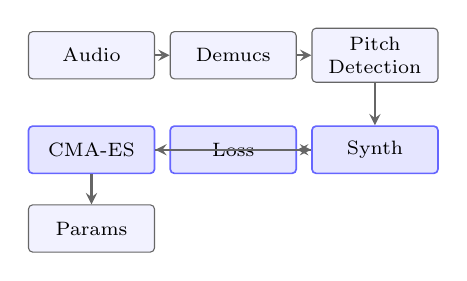
\begin{tikzpicture}[
    node distance=0.9cm,
    box/.style={rectangle, draw=black!60, fill=blue!5, minimum width=1.6cm, minimum height=0.6cm, align=center, rounded corners=1.5pt, font=\scriptsize},
    loopbox/.style={rectangle, draw=blue!60, fill=blue!10, minimum width=1.6cm, minimum height=0.6cm, align=center, rounded corners=1.5pt, font=\scriptsize, line width=0.6pt},
    arr/.style={->, >=stealth, thick, black!60, font=\scriptsize},
]
\node[box] (audio) {Audio};
\node[box, right of=audio, node distance=1.8cm] (demucs) {Demucs};
\node[box, right of=demucs, node distance=1.8cm] (pitch) {Pitch\\Detection};
\node[loopbox, below of=pitch, node distance=1.2cm] (synth) {Synth};
\node[loopbox, left of=synth, node distance=1.8cm] (loss) {Loss};
\node[loopbox, left of=loss, node distance=1.8cm] (cmaes) {CMA-ES};
\node[box, below of=cmaes, node distance=1.0cm] (out) {Params};

\draw[arr] (audio) -- (demucs);
\draw[arr] (demucs) -- (pitch);
\draw[arr] (pitch) -- (synth);
\draw[arr] (synth) -- (loss);
\draw[arr] (loss) -- (cmaes);
\draw[arr] (cmaes) -- (synth);
\draw[arr] (cmaes) -- (out);
\end{tikzpicture}
\caption{Pipeline: audio $\to$ separation $\to$ pitch detection $\to$ CMA-ES optimization loop $\to$ output parameters.}
\label{fig:pipeline}
\end{figure}

\textbf{Pipeline.} Input audio is separated via Demucs~\cite{defossez2021hybrid}, pitch-tracked with TorchCrepe~\cite{kim2018crepe}, segmented into notes, then matched via CMA-ES (Fig.~\ref{fig:pipeline}).

\textbf{Synthesizer.} We implement a 28-parameter differentiable subtractive synthesizer in PyTorch: four oscillator types (saw, pulse with variable width, sine, noise) with 5-voice unison, a sigmoid low-pass filter with variable slope, 2-band parametric EQ, amplitude and filter ADSR envelopes, and delay-line reverb.

\textbf{Loss.} A composite perceptual loss:
\vspace{-2mm}
\begin{equation}
\mathcal{L} = \mathcal{L}_{\text{mel}} + 0.1\,\mathcal{L}_{\text{cent}} + 0.05\,\mathcal{L}_{\text{mfcc}}
\end{equation}
\vspace{-2mm}

\noindent where $\mathcal{L}_{\text{mel}}$ is mel-scaled multi-resolution STFT (FFT sizes 1024, 2048, 8192 with perceptual weighting), $\mathcal{L}_{\text{cent}}$ is normalized spectral centroid distance, and $\mathcal{L}_{\text{mfcc}}$ is MSE over 13 MFCCs.

\textbf{Optimization.} CMA-ES~\cite{hansen2016cmaes} with population 40, $\sigma_0{=}0.15$, and spectral initialization: we analyze the target's rolloff, harmonic ratios, and flatness to set informed starting parameters. Multi-pitch fitting optimizes one patch across three pitches simultaneously.

% ═══════════════ EXPERIMENTS ═══════════════
\section{Experiments \& Results}

\textbf{Target.} A lead synthesizer from a commercial song: 22 notes at three pitches (A3, C\#4, D4), ${\sim}150$\,ms each.

% --- Convergence figure ---
\begin{figure}[t]
\centering
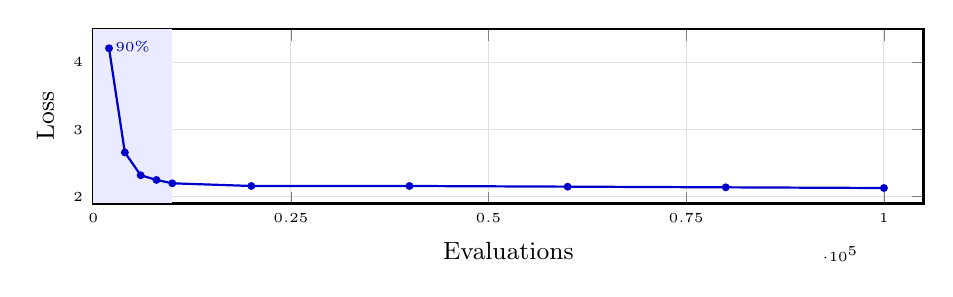
\begin{tikzpicture}
\begin{axis}[
    width=\linewidth, height=3.8cm,
    xlabel={\small Evaluations}, ylabel={\small Loss},
    xmin=0, xmax=105000, ymin=1.9, ymax=4.5,
    xtick={0,25000,50000,75000,100000},
    xticklabel style={font=\tiny},
    yticklabel style={font=\tiny},
    xlabel style={font=\small}, ylabel style={font=\small},
    grid=major, grid style={gray!25}, thick,
]
\fill[blue!8] (axis cs:0,1.9) rectangle (axis cs:10000,4.5);
\node[font=\tiny, text=blue!60!black, anchor=south] at (axis cs:5000,4.0) {90\%};
\addplot[color=blue!80!black, mark=*, mark size=1pt, line width=0.8pt] coordinates {
    (2000,4.21) (4000,2.66) (6000,2.32) (8000,2.25) (10000,2.20)
    (20000,2.16) (40000,2.16) (60000,2.15) (80000,2.14) (100000,2.13)
};
\end{axis}
\end{tikzpicture}
\caption{CMA-ES convergence. 90\% of improvement occurs in the first 10K evaluations (shaded).}
\label{fig:convergence}
\end{figure}

\textbf{Ablation.} Table~\ref{tab:main} shows the progression as we add synth modules. The largest gain comes from unison voices ($-49\%$). Adding unconstrained parameters (29 params) causes CMA-ES to exploit implausible configurations (e.g., detune $=+24$ semitones), degrading results.

\begin{table}[t]
\centering
\small
\caption{Ablation over synthesizer parameters.}
\label{tab:main}
\begin{tabular}{@{}clrc@{}}
\toprule
\textbf{Params} & \textbf{Modules added} & \textbf{Loss} & $\boldsymbol{\Delta}$ \\
\midrule
15 & Osc, filter, ADSR, reverb & 4.60 & -- \\
18 & + unison, noise floor & 2.34 & $-49\%$ \\
24 & + pulse width, filter slope & 2.13 & $-9\%$ \\
28 & + 2-band parametric EQ & \textbf{2.09} & $-2\%$ \\
29 & + distortion, delay, vibrato & \emph{div.} & -- \\
\bottomrule
\end{tabular}
\end{table}

\textbf{Hypothesis testing.} We test eight modifications at 10K evaluations each (Table~\ref{tab:hyp}). Only parametric EQ improves the loss; it allows \emph{boosting} frequencies that a low-pass filter can only cut. The optimizer finds a $+1$\,dB peak at 5.8\,kHz.

\begin{table}[t]
\centering
\small
\caption{Hypothesis tests (10K evals each, baseline loss 2.27).}
\label{tab:hyp}
\begin{tabular}{@{}lr@{}}
\toprule
\textbf{Modification} & \textbf{$\Delta$ Loss} \\
\midrule
Chebyshev waveshaping & $+29\%$ \\
\textbf{Parametric EQ (2 bands)} & $\mathbf{-8\%}$ {\color{green!50!black}$\checkmark$} \\
TFS / envelope loss & $+17\%$ \\
SPSA fine-tuning & $+11\%$ \\
Multi-start CMA-ES ($8{\times}$) & $+29\%$ \\
FM synthesis (2-op) & $+17\%$ \\
\bottomrule
\end{tabular}
\end{table}

\textbf{Convergence.} Fig.~\ref{fig:convergence} shows 90\% of loss reduction in the first 10K evaluations; the remaining 90K yield only marginal gains (${\sim}0.07$), indicating an architectural floor.

% --- Harmonics figure ---
\begin{figure}[t]
\centering
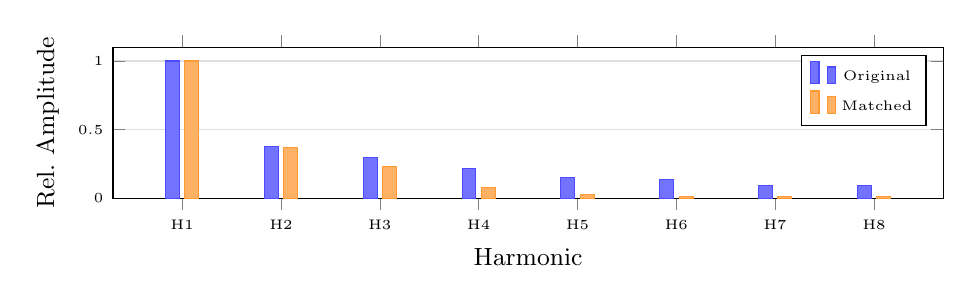
\begin{tikzpicture}
\begin{axis}[
    width=\linewidth, height=3.5cm, ybar, bar width=5pt,
    xlabel={\small Harmonic}, ylabel={\small Rel.\ Amplitude},
    ymin=0, ymax=1.1, xtick=data,
    xticklabels={H1,H2,H3,H4,H5,H6,H7,H8},
    xticklabel style={font=\tiny},
    yticklabel style={font=\tiny},
    xlabel style={font=\small}, ylabel style={font=\small},
    ymajorgrids=true, grid style={gray!25},
    legend style={font=\tiny, at={(0.98,0.95)}, anchor=north east},
    enlarge x limits=0.1,
]
\addplot[fill=blue!55, draw=blue!70] coordinates {(1,1.0)(2,0.38)(3,0.30)(4,0.22)(5,0.15)(6,0.14)(7,0.09)(8,0.09)};
\addlegendentry{Original}
\addplot[fill=orange!60, draw=orange!80] coordinates {(1,1.0)(2,0.37)(3,0.23)(4,0.08)(5,0.03)(6,0.01)(7,0.01)(8,0.01)};
\addlegendentry{Matched}
\end{axis}
\end{tikzpicture}
\caption{Harmonic amplitudes: original vs.\ matched. H1--H3 are closely reproduced; H4--H8 diverge, indicating the architectural floor of subtractive synthesis.}
\label{fig:harmonics}
\end{figure}

\textbf{Spectral analysis.} Fig.~\ref{fig:harmonics} reveals the residual gap: upper harmonics (H4--H8) are 2--5$\times$ weaker in our output. The target exhibits $\text{H3}>\text{H2}$, which is impossible with standard sawtooth or square waveforms, suggesting the original uses FM or wavetable synthesis.

\textbf{Optimizer comparison.} Adam gradient descent plateaus at higher loss (4.60) due to local minima. A PPO-based RL agent (1M steps, 8 parallel environments) matches CMA-ES performance ($4.16 \to 2.31$ in 50 steps) but does not exceed it. CMA-ES with spectral initialization remains the strongest approach.

% ═══════════════ DISCUSSION ═══════════════
\section{Discussion}

\textbf{Why EQ helps.} A low-pass filter can only attenuate; the target has mid-high presence (1--5\,kHz) requiring \emph{boosting}. A 2-band parametric EQ adds this capability with just 4 parameters. This is the only modification that improved our loss across all hypothesis tests.

\textbf{Why more params hurt.} Expanding from 24 to 29 parameters (adding unconstrained distortion, delay, vibrato) allowed CMA-ES to exploit the search space: detune drifted to $+24$ semitones, reverb to 43\%. The optimizer ``cheats'' the loss rather than matching the sound. Constrained, physically meaningful parameters outperform unconstrained expansion.

\textbf{Limitations.} We evaluate on a single target sound with a subtractive synthesizer. The harmonic floor ($\text{H3}>\text{H2}$) suggests FM or wavetable synthesis would extend coverage. The loss plateau at ${\sim}50$K evaluations indicates that improving the loss function (e.g., CDPAM~\cite{manocha2021cdpam}, temporal fine structure) or training a learned encoder may be needed for further gains.

\textbf{Future work.} Supervised encoders, RL agents with shaped rewards, flow-matching generative models over parameter posteriors~\cite{hayes2025flowsynth}, and richer synth architectures are promising directions.

% ═══════════════ REFERENCES ═══════════════
{\small
\bibliographystyle{plainnat}
\bibliography{references}
}

\end{document}
